\subsection{Real Data Preprocessing}
Before real data can be passed to classification algorithm it ought to be preprocessed. 
Peak positions in acquired spectrum differ from measurement to measurement - this problem has been addressed in \cite{Goral2023} master thesis.
Basing on master thesis achievements a function for data preprocessing have been created - \prettyref{lst:data_preprocessing}.

\newenvironment{longlistingF}{\captionsetup{type=listing, width=0.8\textwidth}}{}
\begin{longlistingF}
    \pythoncode{listings/data_preprocessing.py}
    \caption{}
    \label{lst:data_preprocessing}
\end{longlistingF}
\vspace{12pt}

To illustrate its inner workings, a visualization will be used (see \prettyref{fig:spectrum_preprocessing}). The following steps are taken during preprocessing:
\begin{enumerate}
    \item The channels are mapped to energy (work done in \cite{Goral2023}) and cropped if they fall outside the defined range [\texttt{min\_energy}, \texttt{max\_energy}] [KeV] (in the example below, this is not the case).
    \item The left and right boundary, each of size \texttt{energy\_margin} [KeV], is masked with zeros because boundaries tend to have high amount of noise.
    \item The spectrum is padded with zeros until it fills the range [\texttt{min\_energy}, \texttt{max\_energy}].
    \item The spectrum is extrapolated on the left and right sides using the exponential function \texttt{a * np.exp(b * x)}, which is fitted using \texttt{points\_to\_extrapolate\_count} non-zero points at the ends of the spectrum.
    \item Finally, the spectrum is interpolated to the defined length \texttt{target\_length}.
\end{enumerate}

\begin{figure}[H] 
  \centering     
  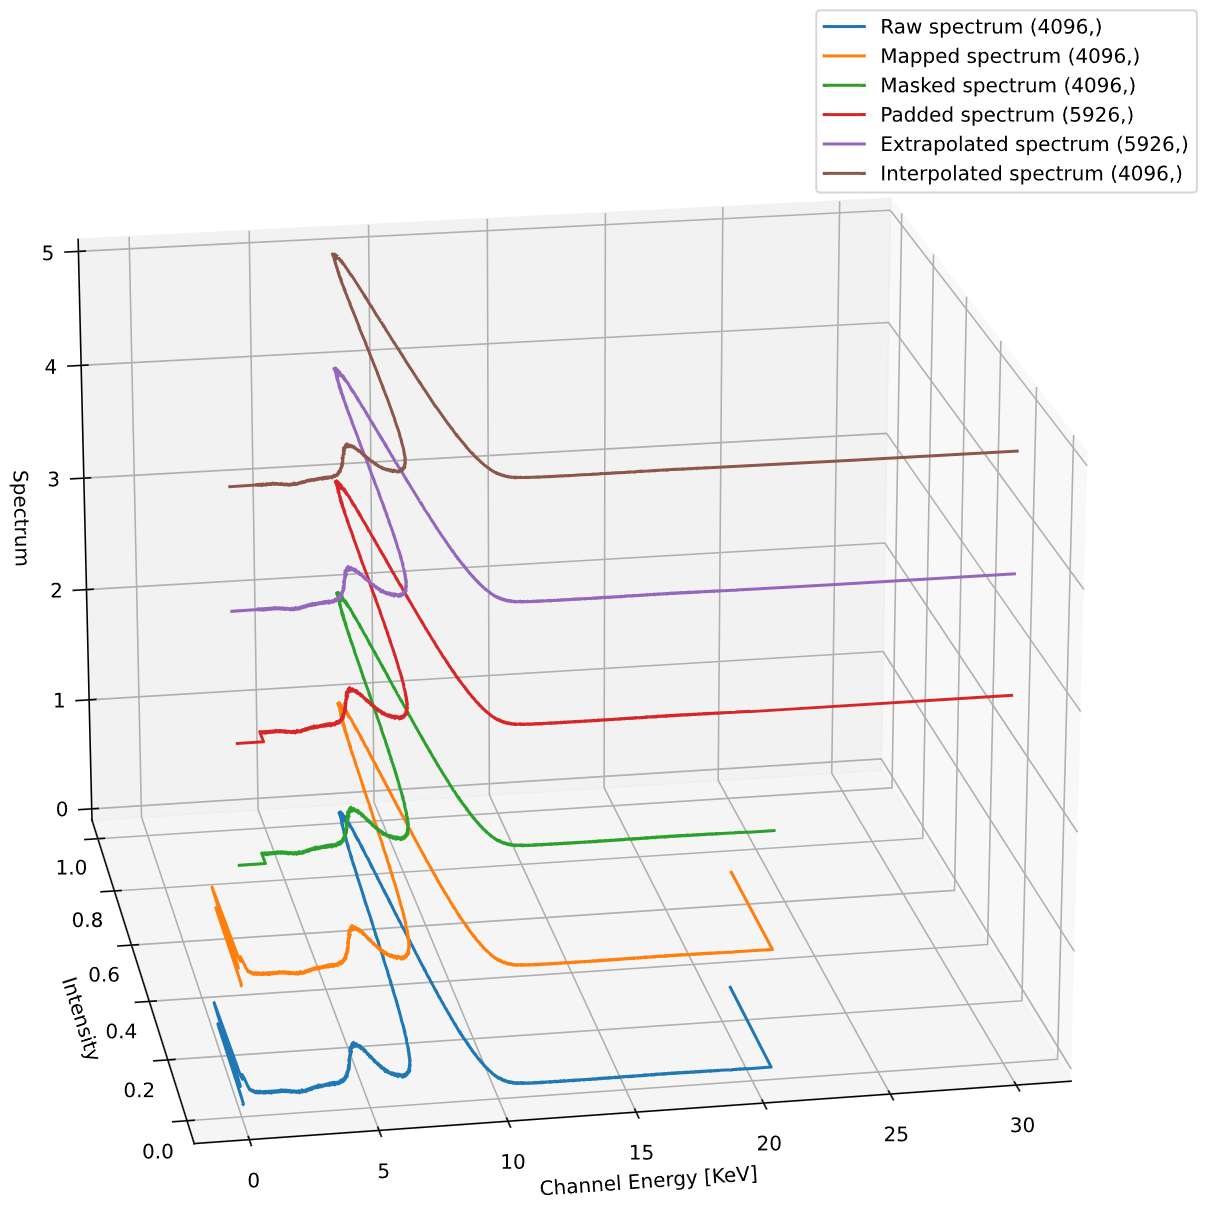
\includegraphics[width=1\textwidth]{img/spectrum_preprocessing.png} 
  \caption{Steps of spectrum preprocessing}
  \label{fig:spectrum_preprocessing}
\end{figure}

The processed spectrum can then be passed to a classifier that was trained using the same energy mapping. 
Alternatively, the extrapolation step can be omitted; in this case, the classifier should also be trained on masked spectra or a different energy range, for example, [1, 29].